\documentclass[12pt]{article}

\usepackage{ceai}
\graphicspath{{../figs/}}

\begin{document}
\doublespacing

\title{CE 488/5588: Applied AI for Engineering\\ \large Topic 14: Generative Deep Learning in Practice --- GANs, VAEs, Diffusion, and Engineering Applications}
\author{}
\date{}
\maketitle

\begin{ch-box}
In Topic 13, we studied the foundations that made deep neural networks practical: stable training, convolution, attention, and the basic intuition behind modern generative models. In this chapter, we shift from \textit{how} these models work to \textit{what they are now used for}. This transition is especially important in engineering, where the value of AI is not only predictive accuracy but also the ability to synthesize designs, generate scenarios, accelerate simulation, reconstruct missing information, and support decision making under uncertainty.

Topic 14 is therefore intentionally application-heavy. The conceptual material here is brief and selective; its purpose is to provide just enough vocabulary to critically read the modern literature on generative AI in engineering. The main emphasis of the chapter will be on use cases, representative workflows, and the practical question every engineer should ask: when does a generative model produce useful structure rather than merely plausible-looking output?
\end{ch-box}

\section{Overview: From Deep Architectures to Generative Engineering Systems}

Classical supervised learning is primarily about prediction. Given an input, we estimate a label, a class probability, or a continuous target. Much of engineering AI has historically followed this pattern: detect cracks, classify faults, predict load, estimate material strength, or forecast traffic speed. Generative AI expands this picture. Instead of only mapping inputs to outputs, we now ask models to \textit{produce} new objects that resemble the patterns in the training data: images, signals, field realizations, shapes, trajectories, candidate layouts, or synthetic operating scenarios.

This change is not merely cosmetic. A discriminative model helps answer questions such as ``What class is this?'' or ``What value should I predict?'' A generative model addresses a different class of questions: ``What could a realistic sample look like?'', ``What missing information is consistent with the observed data?'', or ``What candidate design satisfies desired constraints?'' For engineering, this makes generative models relevant to inverse problems, uncertainty exploration, surrogate scenario generation, data augmentation, digital twins, and automated design support.

At the same time, generative models should not be treated as magic. They learn statistical structure, not physical law by default. Their outputs may be realistic in appearance while violating conservation principles, boundary conditions, manufacturability constraints, or safety requirements. For that reason, this chapter treats generative AI as a powerful modeling tool that must be coupled with domain knowledge, validation, and engineering judgment.

\section*{Learning Objectives}
After completing this chapter, you should be able to:
\begin{itemize}
    \item distinguish discriminative and generative modeling in terms of goals, outputs, and typical engineering use cases;
    \item explain at a high level how VAEs, GANs, and diffusion models differ in training philosophy, output quality, and practical trade-offs;
    \item identify major application areas of generative AI in engineering, including design generation, reconstruction, synthesis, and scientific data augmentation;
    \item evaluate the strengths and limitations of generative AI systems with respect to realism, controllability, data requirements, and physical consistency; and
    \item read application-oriented literature on deep generative models with enough conceptual background to judge whether a method is appropriate for an engineering task.
\end{itemize}

\section{A Short Primer on Generative Models}

\subsection{Discriminative versus Generative Thinking}

A useful starting distinction is between \textbf{discriminative} and \textbf{generative} models. A discriminative model focuses on prediction boundaries or input-output mappings. In the simplest terms, it learns to answer: given $\mathbf{x}$, what is $y$? Logistic regression, support vector machines, most classifiers, and many regression networks are discriminative in this sense. They are optimized to separate classes, estimate labels, or predict targets as accurately as possible.

A generative model aims to represent how the data themselves are distributed, at least well enough to produce new samples or fill in missing structure. Instead of only answering ``what label belongs to this input?'', it tries to answer ``what kinds of inputs are plausible under this data-generating process?'' This makes generation possible, but it also enables related tasks such as denoising, imputation, interpolation, anomaly screening, and conditional synthesis.

For engineers, the distinction is practical rather than philosophical. If the task is to classify bridge damage severity from an image, a discriminative model may be the right tool. If the task is to generate realistic damage scenarios, reconstruct missing sensor fields, create synthetic rare-event data, or produce candidate designs from partial constraints, a generative model becomes attractive.

\begin{alert-box}
\textbf{Engineering perspective:} Discriminative models are often best when the target is fixed and well defined. Generative models become valuable when the task involves synthesis, reconstruction, exploration of alternatives, or reasoning about what the data could have been.
\end{alert-box}

\subsection{Three Main Families: VAE, GAN, and Diffusion}

Modern deep generative modeling is often introduced through three influential families.

\textbf{Variational Autoencoders (VAEs)} learn a compressed latent representation from which new samples can be decoded. They are usually stable to train and useful when we care about smooth latent spaces, interpolation, or representation learning. Their main limitation is that generated outputs may appear overly smooth or less sharp than those of newer methods.

\textbf{Generative Adversarial Networks (GANs)} train two models in competition: a generator tries to produce realistic samples, while a discriminator tries to distinguish generated samples from real ones. GANs became famous for producing sharp, visually impressive outputs, but they can be unstable to train and may suffer from mode collapse, where the generator produces only a limited subset of plausible patterns.

\textbf{Diffusion models} learn to reverse a progressive noising process. Starting from noise, they iteratively denoise until a structured sample emerges. Their major strengths are training stability, high sample quality, and flexibility for conditional generation. Their main drawback is computational cost: generation is typically slower because it requires many iterative steps.

\begin{table}[ht]
\centering
\caption{High-level comparison of common deep generative model families.}
\begin{tabular}{p{0.16\textwidth} p{0.22\textwidth} p{0.24\textwidth} p{0.24\textwidth}}
\toprule
\textbf{Model family} & \textbf{Core idea} & \textbf{Typical strengths} & \textbf{Typical limitations} \\
\midrule
VAE & Encode data into a latent space and decode back to samples & Stable training; useful latent representation; good for interpolation and compression & Outputs may be blurrier or less detailed \\
GAN & Generator and discriminator compete during training & Sharp samples; strong perceptual realism in some domains & Training instability; mode collapse; harder to evaluate \\
Diffusion & Learn to denoise random noise into structured samples & High-quality outputs; stable training; flexible conditioning & Slow sampling; higher computational cost \\
\bottomrule
\end{tabular}
\end{table}

At a high level, one may think of these models as emphasizing different priorities: VAEs emphasize structured representation, GANs emphasize realism, and diffusion models emphasize robust high-quality synthesis. In practice, the best choice depends on the engineering objective. If interpretability of the latent space matters, a VAE may be attractive. If fast high-fidelity image synthesis is the goal, a GAN may still be useful. If quality, flexibility, and state-of-the-art generation matter most, diffusion models are increasingly dominant.

This brief primer is enough for our purposes. The rest of the chapter focuses less on internal architecture details and more on how these model families are being used across engineering domains, what problems they solve well, and where their limitations remain significant.

\section{Generative Models for Engineering Applications}

In many engineering settings, the difficult part is not classification alone but \emph{distribution matching}: generating realistic crack masks from noisy pavement images, reconstructing baseline sensor signals under changing temperatures, or separating structural damage from normal environmental variability. This is where generative models become useful. In Topic 13 we introduced the main model families conceptually; here the emphasis is practical. For civil and infrastructure problems, generative models are rarely used to create photorealistic images for their own sake. Instead, they are used to improve segmentation, augment scarce data, reconstruct normal states, and expose physically meaningful latent factors that support inspection and decision-making.

\subsection{Generative Adversarial Networks (GANs)}

A GAN trains two models in competition: a \emph{generator} that produces synthetic outputs and a \emph{discriminator} that tries to distinguish synthetic outputs from real ones. At a high level, the training objective is a minimax game,
\begin{equation}
    \min_G \max_D \; \mathbb{E}[\log D(x)] + \mathbb{E}[\log(1-D(G(z)))],
\end{equation}
where $G$ tries to generate outputs that look realistic and $D$ tries to detect the fakes. For engineering readers, the most important intuition is not the equation but the consequence: adversarial training penalizes outputs that may be numerically close on average yet look \emph{structurally wrong}. That matters for defects such as cracks, whose thin connected geometry is easy to destroy with ordinary pixel-wise losses.

\begin{figure}[ht]
    \centering
    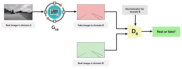
\includegraphics[width=0.8\textwidth]{Topic14fig01.pdf}
    \caption{ICGA architecture for road-surface crack detection. The figure highlights how conditional adversarial learning is paired with a segmentation-style backbone rather than used as unconstrained image generation. Source: \url{https://pmc.ncbi.nlm.nih.gov/articles/PMC8587934/}.}
\end{figure}

\subsection{GANs in Civil Engineering: Crack Detection and Segmentation}

The civil-engineering GAN literature has concentrated heavily on vision problems in which the target class is rare, thin, spatially structured, and easily confused with background clutter. Pavement and road-surface crack detection fit this pattern almost perfectly. Shadows, stains, lane markings, rough texture, and illumination changes all create false positives, while the cracks themselves may be faint, discontinuous, or only partially labeled.

A representative contribution is \emph{CrackGAN} by Zhang, Zhang, and Cheng, which explicitly addressed a practical annotation problem: pavement crack datasets often contain \emph{partially accurate} ground truth rather than clean pixel-perfect masks.\footnote{\url{https://arxiv.org/abs/1909.08216}} Their key observation was that a standard fully convolutional detector trained on imbalanced data can collapse toward the trivial ``all background'' solution. In crack inspection, this is a dangerous failure mode because a model can achieve deceptively good aggregate loss while missing the defect class almost entirely. CrackGAN used adversarial learning to force the model to produce crack-like outputs instead of settling into this degenerate solution. The engineering lesson is important: GANs are attractive not only when data are scarce, but also when \emph{labels are imperfect and class imbalance is severe}. In infrastructure inspection, those conditions are common.

A later and more application-specific example is the conditional GAN pavement segmentation model of Kang and Feng.\footnote{\url{https://pmc.ncbi.nlm.nih.gov/articles/PMC9653803/}} Their framework used a U-net3+-style generator with attention modules and a PatchGAN discriminator, targeting crack segmentation under complex road backgrounds. The conditional setup is especially natural for engineering segmentation: the generator is not inventing an arbitrary image from noise, but mapping a \emph{specific} road image to its crack mask. This matters pedagogically because most engineering GAN use cases are conditional rather than free-form. The model is told, in effect, ``given this noisy measurement, generate the most plausible defect map.'' Kang and Feng reported that adversarial training helped produce smoother, more spatially consistent crack masks on the Crack500 dataset, particularly in the presence of interference such as shadows and bright noise.

\begin{figure}[ht]
    \centering
    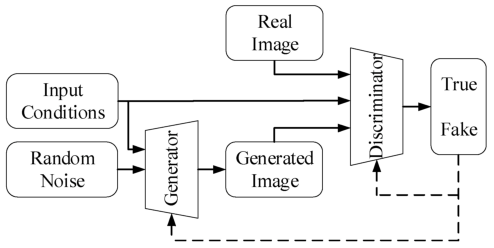
\includegraphics[width=0.82\textwidth]{Topic14fig02.pdf}
    \caption{Conditional GAN structure from a pavement-crack segmentation pipeline. This is representative of how GANs are adapted into practical civil-engineering segmentation systems with task-specific generators and discriminators. Source: \url{https://www.mdpi.com/1424-8220/22/21/8478}.}
\end{figure}

Taken together, these papers show a consistent pattern in civil-engineering GAN adoption. First, GANs are used less as open-ended image generators and more as \emph{structure-preserving regularizers}. The adversarial loss pushes the output toward globally plausible morphology: connected crack traces instead of isolated speckles, cleaner boundaries instead of blurry averages, and more realistic spatial coherence than one typically gets from cross-entropy alone. Second, GANs are often paired with encoder--decoder segmentation backbones such as U-Net variants rather than replacing them. In practice, the CNN performs the heavy lifting of feature extraction, while the GAN objective sharpens the result. Third, the strongest motivation is usually not benchmark novelty but \emph{robustness to messy field conditions}.

At the same time, the literature also reveals recurring pitfalls. GANs are notoriously harder to train than ordinary supervised segmentation networks. Improvements in visual quality do not automatically imply trustworthy defect maps. A GAN can hallucinate plausible-looking crack continuity where the image evidence is weak, which is unacceptable if the model is used for maintenance decisions without human review. In addition, many papers report segmentation metrics under curated datasets, whereas field deployment must confront domain shift: new cameras, new pavement textures, night lighting, water, sealants, and seasonal wear. For this reason, the most convincing civil-engineering use of GANs is not ``GANs generate impressive images,'' but rather ``GANs can improve defect delineation when labels are noisy, defects are thin, and spatial consistency matters.''

\begin{alert-box}
\textbf{Practical takeaway:} In civil infrastructure vision, GANs are most useful when the target is geometrically structured and difficult to label precisely. Their value lies in enforcing realism and spatial coherence, but that same realism pressure can also hide failure modes. Engineering deployment therefore requires careful validation against false negatives, false positives, and out-of-distribution field imagery.
\end{alert-box}

\subsection{Variational Autoencoders (VAEs)}

Where GANs emphasize realism through adversarial competition, VAEs emphasize \emph{structured latent representation}. A VAE learns to compress data into a low-dimensional probabilistic latent space and then reconstruct the input from that space. At a high level, its objective combines two goals:
\begin{equation}
    \mathcal{L}_{\text{VAE}} = \text{reconstruction loss} + \text{latent-space regularization}.
\end{equation}
The first term preserves information needed to reconstruct the signal; the second encourages the latent variables to remain smooth, organized, and sampleable. For engineering applications, that makes VAEs appealing when we care less about photorealistic synthesis and more about learning a compact description of ``normal'' system behavior, environmental variability, or hidden operating states.

\begin{figure}[ht]
    \centering
    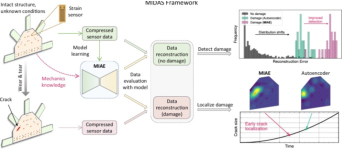
\includegraphics[width=0.72\textwidth]{Topic14fig03.pdf}
    \caption{Overview of a mechanics-informed autoencoder framework for automated structural-damage detection and localization. The pedagogical value is that the latent representation is tied to structural interpretation rather than only to compression. Source: \url{https://www.nature.com/articles/s41467-024-52501-4}.}
\end{figure}

\subsection{VAEs for SHM and Environmental Monitoring}

The most promising VAE-style applications in structural health monitoring (SHM) involve separating damage-sensitive changes from benign environmental and operational variation. This is a central engineering challenge: sensors respond not only to cracks, delamination, corrosion, or stiffness loss, but also to temperature shifts, moisture, traffic, and loading history. A useful latent model should therefore explain ordinary variability without erasing the signature of damage.

A strong recent example is the work of Junges, Lomazzi, Miele, Giglio, and Cadini on ultrasonic guided-wave SHM under changing temperatures.\footnote{\url{https://pmc.ncbi.nlm.nih.gov/articles/PMC10934456/}} Their study is valuable because it targets a realistic nuisance factor rather than an artificial benchmark. In guided-wave monitoring, temperature can alter the measured signal enough to mimic damage or hide it. The authors used a VAE to learn how temperature affects the signal manifold, then reconstruct signals at unseen temperatures. They further introduced a ``forced VAE'' that encouraged a more linear latent-space organization through an additional singular-value-based constraint. Conceptually, this is exactly the kind of role VAEs can play in engineering: not merely compressing data, but \emph{parameterizing environmental variability} so that downstream diagnostics become less temperature-sensitive. The paper is especially instructive because the comparison between the standard VAE and the forced VAE shows that latent spaces are not automatically meaningful; they often need problem-specific structure.

\begin{figure}[ht]
    \centering
    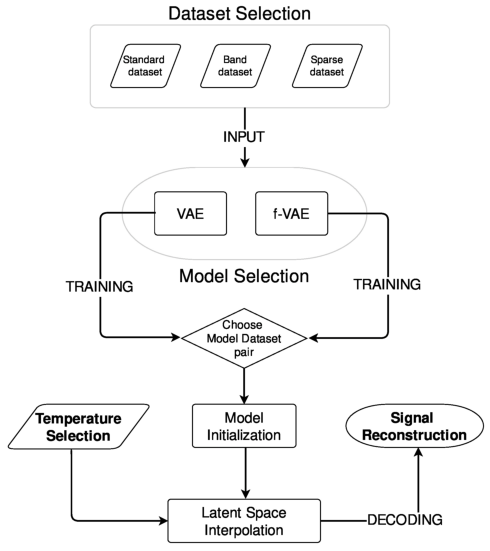
\includegraphics[width=0.74\textwidth]{Topic14fig04.pdf}
    \caption{Workflow for training and signal generation in a VAE-based structural-health-monitoring pipeline under temperature variation. This figure is useful because it makes the environmental-variability problem concrete. Source: \url{https://www.mdpi.com/1424-8220/24/5/1494}.}
\end{figure}

A second approved example, although not a classical VAE in the strict sense, points in the same direction and is worth discussing here because it clarifies where this literature is heading. Li et al.\ developed MIDAS, a mechanics-informed autoencoder for automated detection and localization of unforeseen structural damage.\footnote{\url{https://arxiv.org/abs/2402.15492}} Their model embeds mechanical structure into the latent representation and reports improved performance relative to a standard autoencoder, including better sensitivity to minor damage. The reason this paper matters for a VAE discussion is methodological: the broader autoencoder family in SHM is moving away from purely generic latent compression and toward \emph{physics-aware latent spaces}. For civil engineers, this is likely more important than the exact acronym. Whether the architecture is a standard autoencoder, a VAE, or a hybrid latent model, the central question is the same: does the latent space align with the mechanics of the structure and the nuisance variables of the environment?

These studies suggest three broader themes. First, VAEs are especially well matched to \emph{baseline modeling} problems. In SHM, one often has abundant data from healthy states and very limited data from damaged states. A VAE can learn what normal signals look like and flag departures through reconstruction mismatch or latent-space shifts. Second, VAEs are useful when environmental effects are continuous rather than categorical. Temperature does not switch between a few discrete classes; it moves continuously, making a smooth latent manifold appealing. Third, the best engineering results come when the latent model is not treated as a black box. Junges et al.\ explicitly shaped the latent space for temperature interpolation, and Li et al.\ injected mechanical knowledge. Both moves reflect an engineering principle: latent variables should correspond, as much as possible, to interpretable sources of variation.

The limitations are equally important. VAEs often produce overly smooth reconstructions, which can suppress weak but important damage signatures. If the latent model is trained too aggressively on ``normal'' variability, it may absorb early-stage defects as harmless variation. Conversely, if the latent space is poorly regularized, interpolation across environmental conditions may be unreliable. For deployment, the practical challenge is not just anomaly scoring but \emph{what kind of anomaly the model has learned to ignore}. This is why domain knowledge, sensor physics, and operating-condition metadata remain essential.

\begin{alert-box}
\textbf{Practical takeaway:} In SHM and related monitoring problems, VAEs are valuable because they can model normal variability in a compact latent space. Their real engineering promise is not generic data generation, but the ability to disentangle environmental effects from damage-sensitive behavior---especially when the latent space is constrained by physics or by known operating trends such as temperature.
\end{alert-box}

\subsection{Diffusion Models: From Noise to Controlled Generation}

Diffusion models became the dominant image-generation paradigm because they separate a difficult task---``create a realistic image''---into many easier tasks: remove a small amount of noise, then repeat. Conceptually, the model is trained by corrupting real data step by step until the data become nearly random noise, and then learning the reverse process. Generation therefore becomes an iterative refinement procedure: begin with noise, then gradually denoise toward a coherent sample.

This sounds computationally expensive---and it is---but it brings two major advantages. First, the training problem is much more stable than the adversarial game used in GANs. Second, the iterative process is naturally compatible with \emph{conditioning}: the denoising trajectory can be guided by text, sketches, masks, or layout constraints. That conditioning ability is what made diffusion models central to modern generative AI. Systems such as DALL-E, Midjourney, and Stable Diffusion popularized the idea that a user could specify a desired image in natural language and obtain multiple plausible visual realizations.

At a high level, diffusion is therefore best understood not as ``magic image creation,'' but as \textbf{constrained iterative generation}. This is especially relevant for engineering, where the goal is rarely unconstrained creativity; instead, one wants to generate alternatives that satisfy geometry, boundary conditions, functional requirements, or textual specifications.

\subsection{Diffusion Applications in Civil Engineering and the Built Environment}

The built environment is a particularly natural application area for diffusion models because many design tasks are constrained generation problems. A floor plan, site concept, facade arrangement, or interior layout is not an arbitrary image; it must satisfy geometry, adjacency, access, circulation, and programmatic requirements. Diffusion models are attractive precisely because they can generate \emph{many} candidates while conditioning on such constraints.

A clear example is recent work on \emph{floorplan generation via latent diffusion}, where the model takes inputs such as a lot footprint and a textual description of building functionality, then produces candidate floor plans for different building types.\footnote{\url{https://arxiv.org/abs/2412.06859}} This is pedagogically useful because it shows diffusion in its most intuitive engineering form: the model is not merely painting a pretty image, but mapping boundary conditions and semantic requirements into spatial layouts. The value is not only automation; it is rapid exploration of alternatives under partial specification.

\begin{figure}[ht]
    \centering
    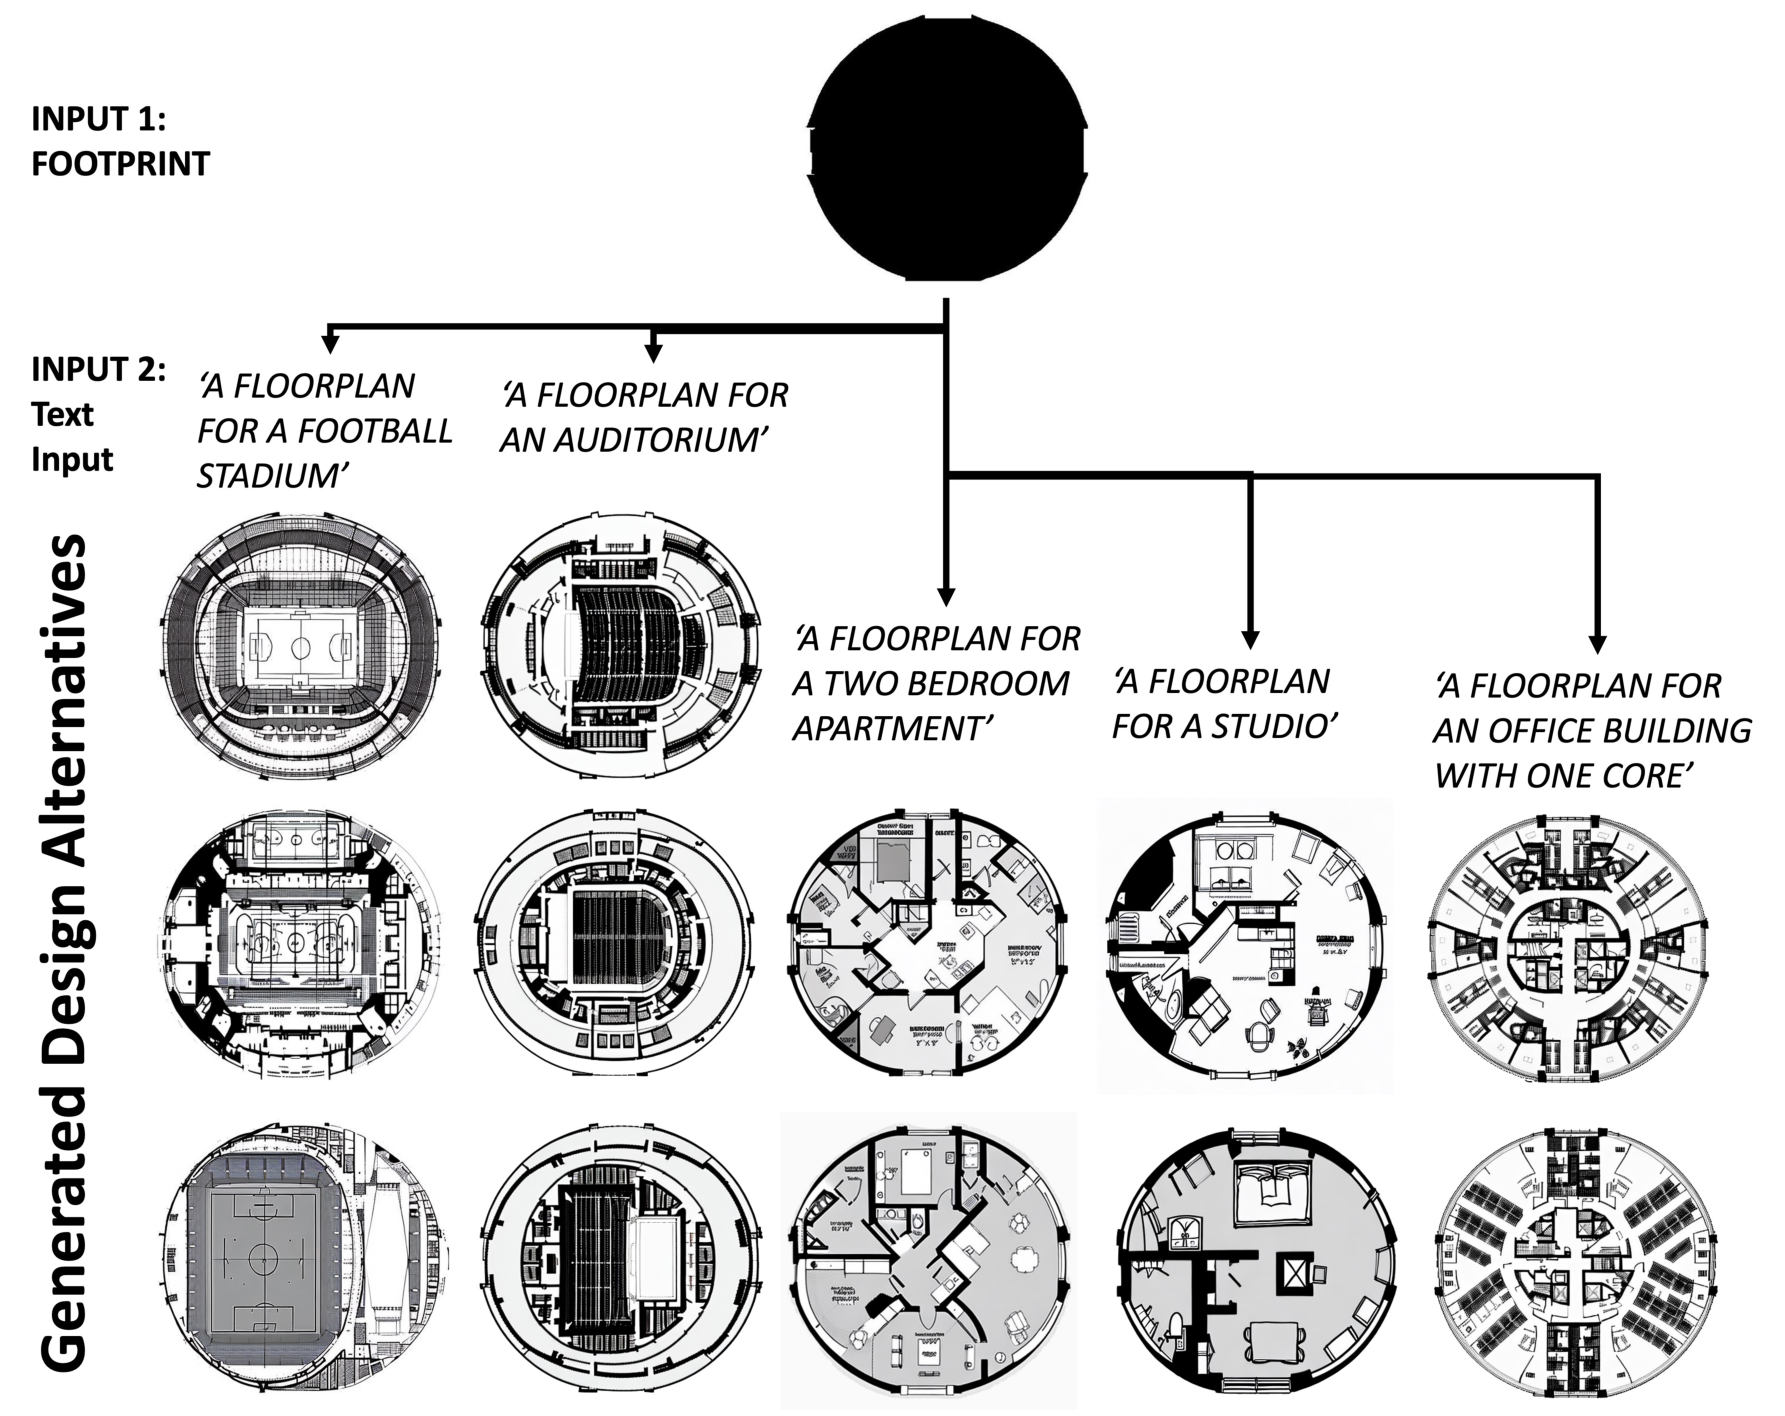
\includegraphics[width=0.82\textwidth]{Topic14fig05.pdf}
    \caption{Latent-diffusion floorplan generation conditioned on lot footprint and textual description. This is an accessible example of controlled diffusion generation in the built environment. Source: \url{https://arxiv.org/abs/2412.06859}.}
\end{figure}

An even more engineering-relevant example is \emph{DiffPlanner}, a recent vector floor-plan generation approach.\footnote{\url{https://arxiv.org/abs/2508.13738}} Its importance is conceptual as much as technical. Many image-generation pipelines operate in raster space: they produce pixels first, then require post-processing to recover geometry. DiffPlanner instead works directly with vector-style representations and decomposes the process into design-relevant stages such as room-node prediction, adjacency relationships, bubble-diagram formation, and partitioning. This is much closer to how designers and engineers already think. It suggests a path from generative AI toward CAD/BIM-compatible workflows rather than purely illustrative outputs.

\begin{figure}[ht]
    \centering
    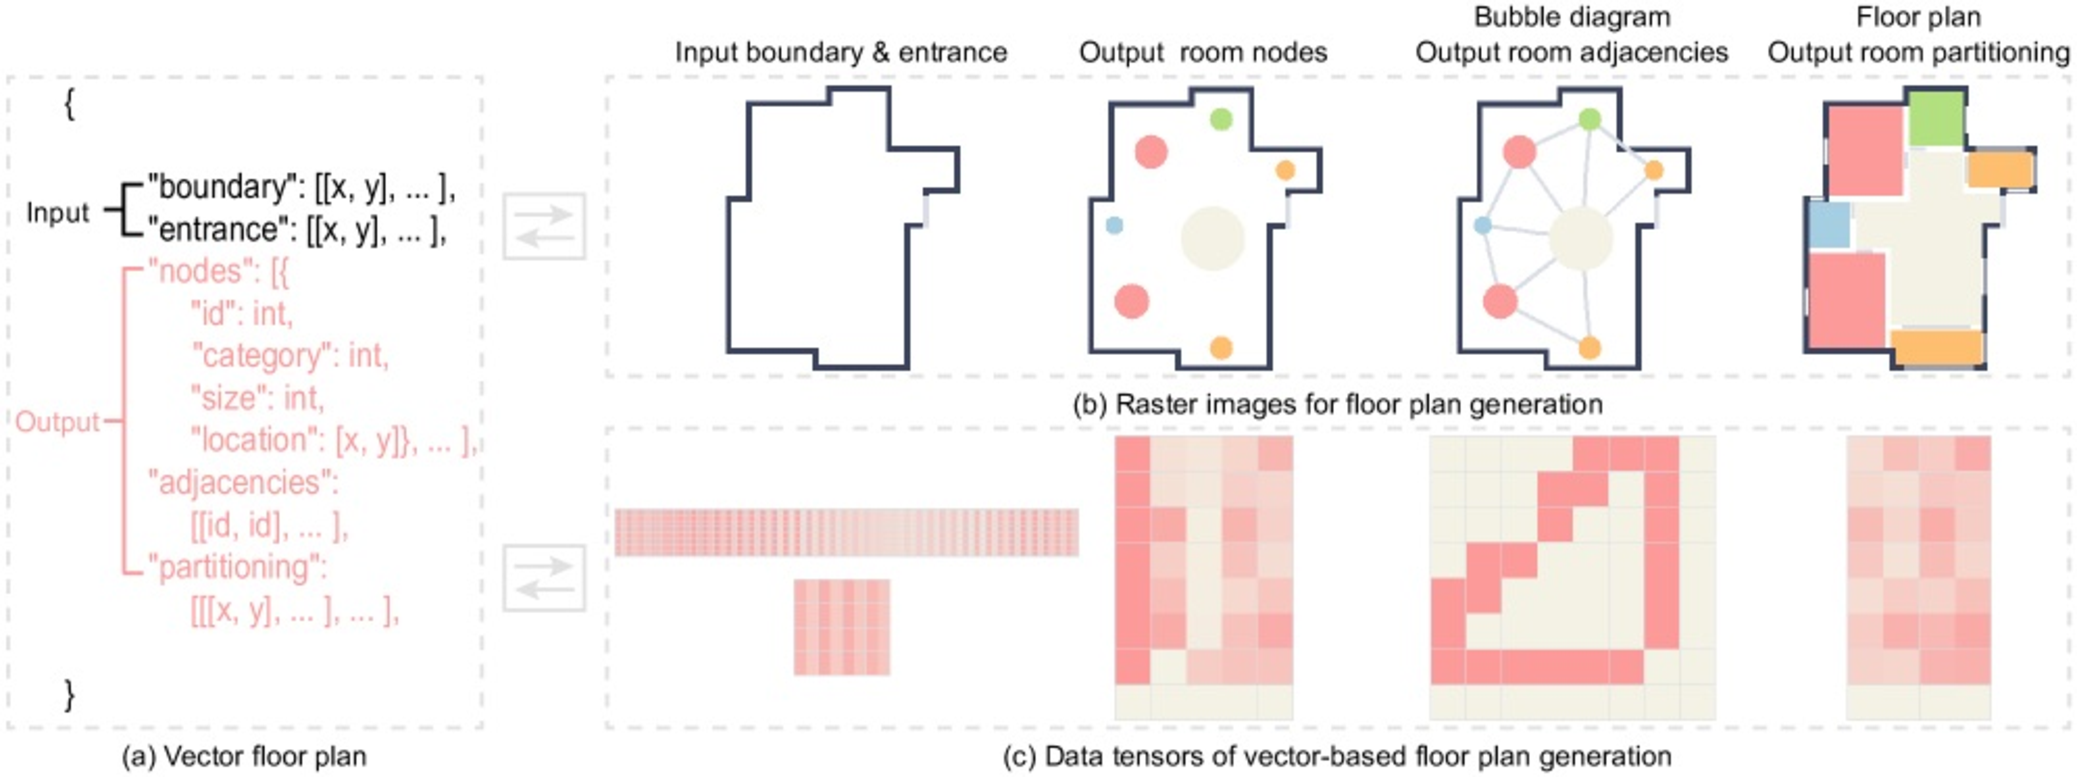
\includegraphics[width=0.86\textwidth]{Topic14fig06.pdf}
    \caption{DiffPlanner overview comparing raster-based floorplan generation with a direct vector-space workflow. This figure is especially useful for explaining why structured engineering outputs differ from ordinary image synthesis. Source: \url{https://arxiv.org/abs/2508.13738}.}
\end{figure}

These examples point to several broader civil-engineering opportunities:
\begin{itemize}
    \item \textbf{Early-stage design exploration.} Generate multiple plan or layout alternatives from footprints, zoning constraints, program descriptions, or circulation objectives.
    
    \item \textbf{Human-in-the-loop concept development.} Use diffusion to propose options, while engineers or architects evaluate code compliance, constructability, cost, and performance.
    
    \item \textbf{Scenario visualization.} Create plausible visualizations of infrastructure states, retrofits, flood impacts, or construction staging to support planning and communication.
    
    \item \textbf{Synthetic training data.} Generate rare or costly visual cases---for example, unusual damage patterns or edge-case built-environment scenes---to augment downstream datasets.
\end{itemize}

At the same time, engineering use requires caution. A visually plausible floor plan is not automatically a valid one. Structural systems, egress, accessibility, MEP coordination, and code requirements impose hard constraints that purely visual generation may ignore. Thus, in civil engineering, diffusion models are best interpreted as \textbf{proposal engines} rather than decision engines. Their role is to expand the design space and accelerate iteration, not to replace engineering judgment.

\subsection{Social Hype, Media Visibility, and Broader Implications}

Diffusion models became visible to the general public much faster than GANs or VAEs because their outputs were immediately legible and shareable. A text prompt could produce a polished illustration, a photorealistic scene, or a stylized rendering in seconds. This made image generation \emph{viral} on social media platforms: users did not need to understand the model architecture to appreciate the result. The technology therefore diffused socially as well as computationally.

That visibility has important implications:
\begin{itemize}
    \item \textbf{Viral image generation and aesthetic democratization.} Diffusion tools lowered the barrier to producing visually persuasive content. For design ideation and communication, this is powerful. For public discourse, it also means polished images can spread faster than verification.
    
    \item \textbf{Misinformation and fabricated disaster imagery.} During floods, earthquakes, wildfires, or other crises, generated images can depict scenes that never occurred but are emotionally convincing. For engineers, planners, and emergency managers, this creates a new information-quality problem: visual evidence can no longer be treated as inherently trustworthy.
    
    \item \textbf{Deepfakes and identity misuse.} Although deepfakes are not limited to diffusion, diffusion-based generation and editing have improved realism in faces, voices, and videos. This raises concerns about consent, impersonation, and the erosion of trust in digital media.
    
    \item \textbf{Text-to-video hype.} Recent text-to-video systems extended the public excitement from still images to dynamic scenes. The hype is understandable: video appears closer to ``world simulation.'' But the same concerns scale up as well---fabricated evidence, synthetic events, and persuasive but false visual narratives.
\end{itemize}

For an engineering audience, the key lesson is not simply that generative AI is exciting or dangerous. It is that \textbf{synthetic media changes the evidentiary status of images and videos}. In domains such as infrastructure inspection, disaster response, or public communication, trustworthy provenance, metadata, and validation become as important as generation quality.

\section{Comparing GANs, VAEs, and Diffusion Models}

GANs, VAEs, and diffusion models all address the same broad goal---learning a data distribution well enough to generate new samples---but they do so with very different trade-offs.

\begin{table}[ht]
    \centering
    \small
    \begin{tabulary}{\textwidth}{@{} L L L L @{}}
        \toprule
        \textbf{Property} & \textbf{GANs} & \textbf{VAEs} & \textbf{Diffusion Models} \\
        \midrule
        \textbf{Core idea} & Generator fools discriminator & Encode/decode through latent space & Reverse a gradual noising process \\
        \textbf{Strength} & Sharp, realistic samples; fast inference & Structured latent representation; efficient sampling & High fidelity, diverse outputs, strong conditioning \\
        \textbf{Typical weakness} & Unstable training; mode collapse & Blurrier outputs; oversmoothing & Slow generation; high compute cost \\
        \textbf{Best use case} & When realism and speed both matter & When latent-space interpolation/compression matters & When quality, controllability, and diversity matter most \\
        \textbf{Engineering interpretation} & Good for targeted synthesis if training is stable & Good for low-dimensional representations and anomaly-style reasoning & Good for constrained design exploration and multimodal generation \\
        \bottomrule
    \end{tabulary}
    \caption{High-level comparison of the three major generative model families.}
\end{table}

A useful summary is the following:
\begin{itemize}
    \item \textbf{GANs} are often the most visually sharp, but they are also the most temperamental to train. The generator and discriminator must remain in balance; if one dominates, learning becomes unstable.
    
    \item \textbf{VAEs} are conceptually elegant because they learn a continuous latent space. This makes them useful for interpolation, compression, and representation learning, but the generated outputs can appear blurrier than those from GANs or diffusion.
    
    \item \textbf{Diffusion models} are currently the most flexible and controllable for high-quality generation. Their main price is computational: denoising is iterative, so inference is slower and more expensive.
\end{itemize}

From an engineering standpoint, the comparison is not about declaring a universal winner. It is about matching the model family to the problem:
\begin{itemize}
    \item If one needs \textbf{fast generation} and can tolerate training difficulty, GANs remain relevant.
    \item If one needs an interpretable \textbf{latent representation} for variation, interpolation, or anomaly analysis, VAEs remain useful.
    \item If one needs \textbf{high-quality conditioned generation} from text, masks, layouts, or multimodal specifications, diffusion is currently the strongest general-purpose choice.
\end{itemize}

Several challenges remain across all three families:
\begin{itemize}
    \item \textbf{Constraint satisfaction.} Generated outputs may look plausible while violating physics, codes, or functional requirements.
    \item \textbf{Evaluation difficulty.} ``Good-looking'' is not the same as useful, valid, or trustworthy.
    \item \textbf{Data bias.} Models inherit the biases and gaps of their training sets.
    \item \textbf{Compute and sustainability.} Large generative models are expensive to train and deploy.
    \item \textbf{Trust and provenance.} As synthetic content improves, distinguishing authentic from generated artifacts becomes harder.
\end{itemize}

\section{Conclusion}

This chapter examined generative deep learning through three complementary model families. \textbf{GANs} introduced the adversarial paradigm and demonstrated that neural networks could generate highly realistic samples, but at the cost of difficult and often unstable training. \textbf{VAEs} provided a principled latent-space view of generation, offering a smoother and more interpretable representation of variation. \textbf{Diffusion models} then emerged as the most influential recent approach, combining training stability, high sample quality, and strong conditioning capability.

For engineering students, the most important takeaway is that these models are not merely tools for making synthetic pictures. They are increasingly becoming interfaces for \textbf{design exploration}, \textbf{scenario generation}, and \textbf{human-AI collaboration}. At the same time, their outputs must be interpreted critically: realism is not validity, and generative fluency is not engineering correctness.

Notice also what made diffusion models socially transformative: they connected generation to \emph{language-like prompts}. A user could specify intent in words and receive images, layouts, or videos as outputs. That observation leads naturally to the next topic. To understand why prompting works, why text has become the control interface for modern AI, and how large models learn meaning from language at scale, we next turn to \textbf{natural language processing, Transformers, and large language models} in Topic 15.

\end{document}
